%!TEX root = main_ISMB.tex
\section{Supplementary data}
\subsection{Benchmark \ourprog vs \RNAinverse}
Using the same dataset of $50$ structures, we generated $100$ samples
per structure with \RNAinverse. They yield for most parameters
a high entropy.
Table.~\ref{tab:nb_rnainv} contains the number of samples with a given \GCContent generated by \RNAinverse. The vast majority resides around $50\%-70\%$, showing one of its major deficiencies. 
 For all structures that have been solved 
by the three methods, only \RNAinverse, only \texttt{Incarnation} and
\texttt{Incarnation} followed by \RNAinverse, 
we present for every different concentration of \GCContent
the average sample entropy and the average base pairs entropy in Figure.~\ref{fig:rnainverse}.

\begin{table}[h!]
	\begin{center}
		\begin{tabular}{|c|ccccc|}
		\hline
		Target \GCContent & 10 & 30 & 50 & 70 & 90\\ \hline
   $\#$\RNAinverse samples& 11 & 437 & 3362 & 1155 & 35\\ \hline
		\end{tabular}
	\end{center}
  \caption{Overall \GCContent distribution for sequences designed using \RNAinverse.}
	\label{tab:nb_rnainv}
\end{table}


\begin{figure}[ht!]
	\centering
	%\hspace{-5em}
	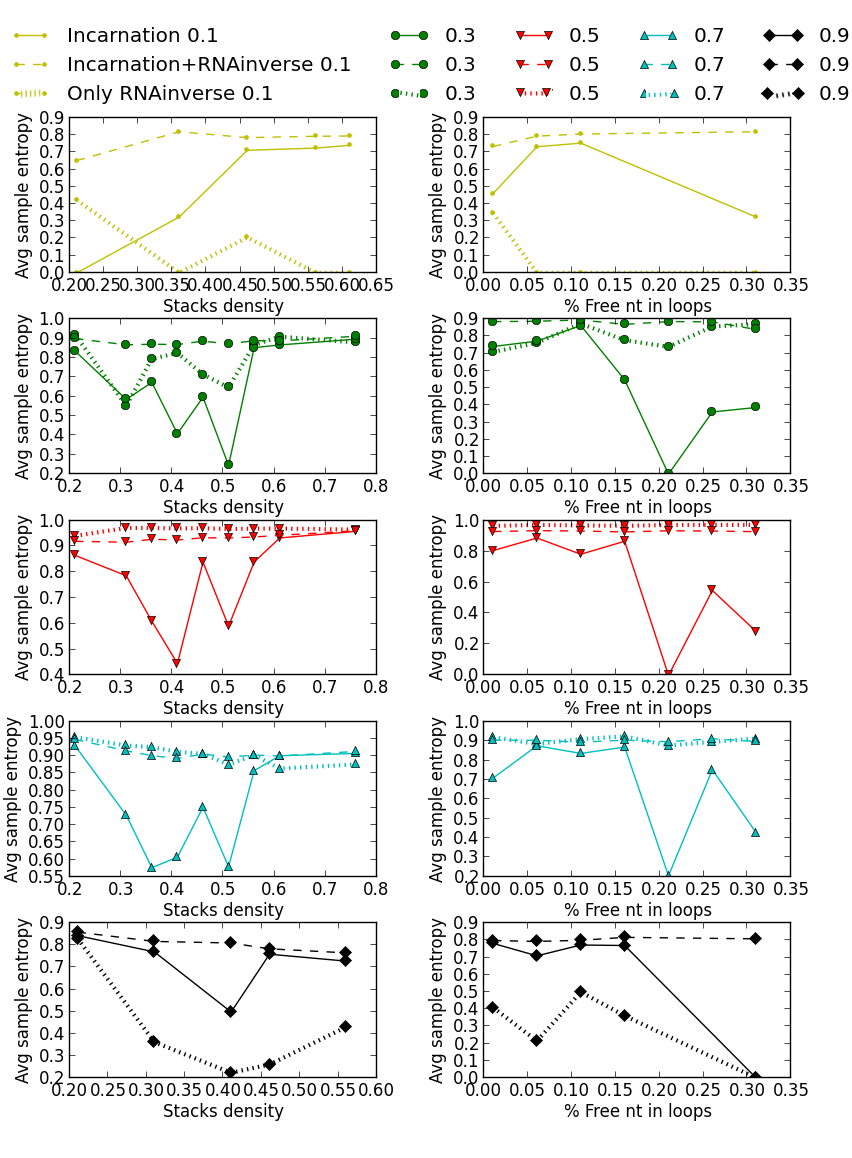
\includegraphics[width=0.5\textwidth]{Figures/RNAinverse_data_100.png}
	\caption{Entropy and \GCContent  for structures solved by
	the 3 methods.}
	\label{fig:rnainverse}
\end{figure}
{\em Récupérer Base-pair entropy}


%The same analysis but only for structures solved by \texttt{Incarnation}
%and \texttt{Incarnation} followed by \RNAinverse, is presented in 
%Fig.~\ref{fig:inc_rnainv}
%
%\begin{figure}
%	\centering
%	\includegraphics{}
%	\caption{Entropy and \texttt{C+G} content for structures solved by
%	the \texttt{Incarnation} and \texttt{Incarnation}$+$\RNAinverse.}
%	\label{fig:inc_rnainv}
%\end{figure}
\subsection{Limited impact on \GC of local-search postprocessing of \ourprog output}
Since local search approaches tend to experience a bias towards \GC{}-rich regions, it could be expected that our glocal approach, by postprocessing unpaired regions using a local search algorithm, would suffer from such a drift.
However, as summarized in Table~\ref{table:impact_on_gc}, we observed that the local search heuristic used to design nucleotides in loop regions has a very limited impact on the \GCContent. For each class of \GCContent, we reported the observed \GCContent in the sequence initially generated by \ourprog, and the observed \GCContent after the \RNAinverse postprocessing (as defined in Section \ref{subsec:glocal_method}). Our results show that the \GCContent is relatively well conserved (less than 6\% variation), with a general tendency of the postprocessing step to bring the \GCContent back to 50\%. 

\begin{table}[h!]
\begin{center}
\resizebox{0.5\textwidth}{!}{
\begin{tabular}{|c|c|c|}
\hline
\multirow{3}{*}{Target \GCContent (\%)}& \multicolumn{2}{|c|}{Designed sequences \GCContent (\%)}\\ \cline{2-3}
 & \ourprog & \ourprog + \RNAinverse\\
 & (Global) & ({Glocal}) \\
\hline
10\% & 15\% & 21\% \quad $\nearrow 6\%$\\
30\% & 30\% & 33\% \quad $\nearrow 3\%$\\
50\% & 48\% & 49\% \quad $\nearrow 1\%$\\
70\% & 71\% & 69\% \quad $\searrow 2\%$\\
90\% & 83\% & 78\% \quad $\searrow 5\%$\\
\hline
\end{tabular}
}
\end{center}
\caption{Observed \GCContent of solutions returned by \ourprog (2nd column) and after the application of the local search postprocessing (3rd column).}
\label{table:impact_on_gc}
\end{table}
